\section{Алгоритм нахождения самопересечений} \label{ch3:selfCollision}
	Как было сказано ранее в главе \ref{ch2:pbd-improvments}, авторами оригинальной статьи уже был предложен алгоритм обнаружения самоперечений, однако построение сложной структуры представленной в \cite{teschner2003optimized} является слишком долгой операцией на GPU, особенно для систем симуляции реального времени. В связи с этим, был разработан и реализован другой алгоритм обнаружения самопересечений.
	
	Во-первых: вместо обработки пересечений частиц и треугольников, было принято решение реализовать обработку перечений двух частиц, где каждая частица задавалась как сфера. При этом, радиусы упомянутых сфер выбираются таким образом, чтобы они были не меньше чем половина длины покоя струтурного ограничения. Помимо этого, самопересечение между частицами, соединенными структурными ограничениями, или растяжениями сдвига - не проверяются, так как их положение уже задается при помощи ограничений.
	
	Во-вторых: для обнаружения соседних частиц, используется алгоритм пространственного хеширования\cite{hashing2023}. Идея данного алгоритма заключается в создании двух массивов: первый $HashMap$ будет для каждой ячейки пространства хранить индекс в массиве $Pointers$ соответствующий первому из элементов лежащих в данной ячейке. Таким образом, для того чтобы перебрать все элементы принадлежащие данной ячейке пространства, достаточно получить индекс в массиве $HashMap$ (назовем этот индекс $hash$), а затем пройтись по элементам $Pointers$ от $HashMap[hash]$ (включительно), до $HashMap[hash + 1]$ (не включительно). Преимуществом данного алгоритма является то, что для построения данной хеш-таблицы не требуется сортировок, или других сложнопараллелизируемых задач, вместо них в данном алгоритме применяется лишь префиксная сумма, для которой уже разработаны алгоритмы параллельного обсчёта (например представленный в \cite{hillis1986data}). Недостатком данной хеш-таблицы является то, что она не имеет возможности динамического добавления и удаления, однако в рамках данной задачи это не требуется.
	
	В третьих, вместо того, чтобы записывать в хеш-таблицу частицы лежащие в соответствующей ячейке пространства, было принято решение записывать не только лежащие в соответствующей ячейке пространства, но и в соседних ячейках. Данное изменение не влияет на объем памяти занимаемый хеш таблицей, но позволяет существенно уменьшить количество обращений к глобальной памяти на этапе обработки соседних вершин.
	
		
	\begin{figure}[ht!] 
		\center
		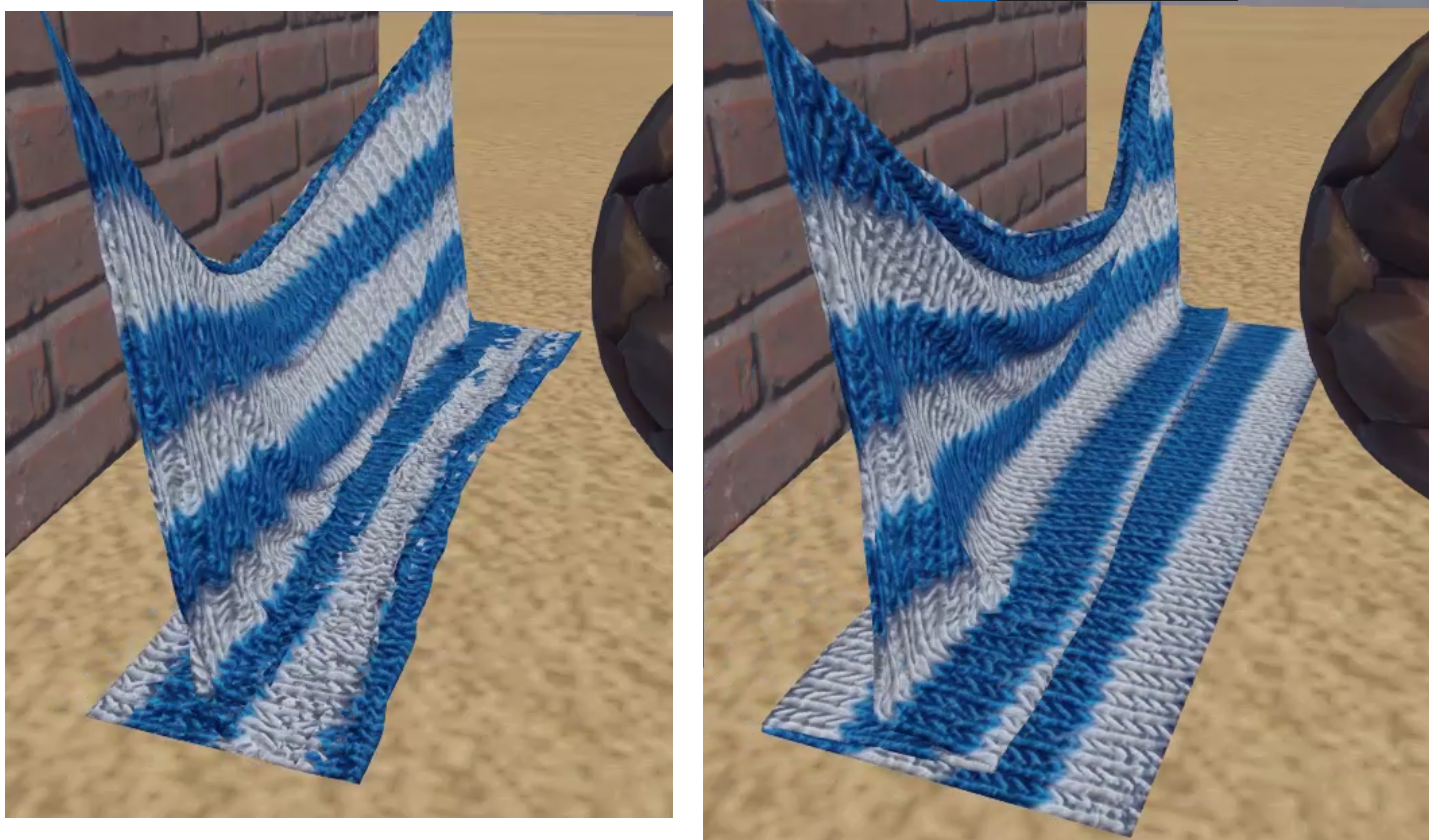
\includegraphics [scale=0.4] {my_folder/images//selfCollisionOffOn}
		\caption{Сравнение поведения симуляционной ткани с алгоритмом самопересечения и без. На рисунке слева проверка самопересечений не производится, а на рисунке справа используется описанный алгоритм.}
		\label{fig:selfCollision}  
	\end{figure}	
	\FloatBarrier

%% Вспомогательные команды - Additional commands
%
%\newpage % принудительное начало с новой страницы, использовать только в конце раздела
%\clearpage % осуществляется пакетом <<placeins>> в пределах секций
%\newpage\leavevmode\thispagestyle{empty}\newpage % 100 % начало новой страницы